% Options for packages loaded elsewhere
\PassOptionsToPackage{unicode}{hyperref}
\PassOptionsToPackage{hyphens}{url}
\PassOptionsToPackage{dvipsnames,svgnames,x11names}{xcolor}
%
\documentclass[
  authoryear,
  preprint,
  1p]{elsarticle}

\usepackage{amsmath,amssymb}
\usepackage{iftex}
\ifPDFTeX
  \usepackage[T1]{fontenc}
  \usepackage[utf8]{inputenc}
  \usepackage{textcomp} % provide euro and other symbols
\else % if luatex or xetex
  \usepackage{unicode-math}
  \defaultfontfeatures{Scale=MatchLowercase}
  \defaultfontfeatures[\rmfamily]{Ligatures=TeX,Scale=1}
\fi
\usepackage{lmodern}
\ifPDFTeX\else  
    % xetex/luatex font selection
\fi
% Use upquote if available, for straight quotes in verbatim environments
\IfFileExists{upquote.sty}{\usepackage{upquote}}{}
\IfFileExists{microtype.sty}{% use microtype if available
  \usepackage[]{microtype}
  \UseMicrotypeSet[protrusion]{basicmath} % disable protrusion for tt fonts
}{}
\makeatletter
\@ifundefined{KOMAClassName}{% if non-KOMA class
  \IfFileExists{parskip.sty}{%
    \usepackage{parskip}
  }{% else
    \setlength{\parindent}{0pt}
    \setlength{\parskip}{6pt plus 2pt minus 1pt}}
}{% if KOMA class
  \KOMAoptions{parskip=half}}
\makeatother
\usepackage{xcolor}
\setlength{\emergencystretch}{3em} % prevent overfull lines
\setcounter{secnumdepth}{5}
% Make \paragraph and \subparagraph free-standing
\makeatletter
\ifx\paragraph\undefined\else
  \let\oldparagraph\paragraph
  \renewcommand{\paragraph}{
    \@ifstar
      \xxxParagraphStar
      \xxxParagraphNoStar
  }
  \newcommand{\xxxParagraphStar}[1]{\oldparagraph*{#1}\mbox{}}
  \newcommand{\xxxParagraphNoStar}[1]{\oldparagraph{#1}\mbox{}}
\fi
\ifx\subparagraph\undefined\else
  \let\oldsubparagraph\subparagraph
  \renewcommand{\subparagraph}{
    \@ifstar
      \xxxSubParagraphStar
      \xxxSubParagraphNoStar
  }
  \newcommand{\xxxSubParagraphStar}[1]{\oldsubparagraph*{#1}\mbox{}}
  \newcommand{\xxxSubParagraphNoStar}[1]{\oldsubparagraph{#1}\mbox{}}
\fi
\makeatother


\providecommand{\tightlist}{%
  \setlength{\itemsep}{0pt}\setlength{\parskip}{0pt}}\usepackage{longtable,booktabs,array}
\usepackage{calc} % for calculating minipage widths
% Correct order of tables after \paragraph or \subparagraph
\usepackage{etoolbox}
\makeatletter
\patchcmd\longtable{\par}{\if@noskipsec\mbox{}\fi\par}{}{}
\makeatother
% Allow footnotes in longtable head/foot
\IfFileExists{footnotehyper.sty}{\usepackage{footnotehyper}}{\usepackage{footnote}}
\makesavenoteenv{longtable}
\usepackage{graphicx}
\makeatletter
\newsavebox\pandoc@box
\newcommand*\pandocbounded[1]{% scales image to fit in text height/width
  \sbox\pandoc@box{#1}%
  \Gscale@div\@tempa{\textheight}{\dimexpr\ht\pandoc@box+\dp\pandoc@box\relax}%
  \Gscale@div\@tempb{\linewidth}{\wd\pandoc@box}%
  \ifdim\@tempb\p@<\@tempa\p@\let\@tempa\@tempb\fi% select the smaller of both
  \ifdim\@tempa\p@<\p@\scalebox{\@tempa}{\usebox\pandoc@box}%
  \else\usebox{\pandoc@box}%
  \fi%
}
% Set default figure placement to htbp
\def\fps@figure{htbp}
\makeatother

\makeatletter
\@ifpackageloaded{caption}{}{\usepackage{caption}}
\AtBeginDocument{%
\ifdefined\contentsname
  \renewcommand*\contentsname{Table of contents}
\else
  \newcommand\contentsname{Table of contents}
\fi
\ifdefined\listfigurename
  \renewcommand*\listfigurename{List of Figures}
\else
  \newcommand\listfigurename{List of Figures}
\fi
\ifdefined\listtablename
  \renewcommand*\listtablename{List of Tables}
\else
  \newcommand\listtablename{List of Tables}
\fi
\ifdefined\figurename
  \renewcommand*\figurename{Figure}
\else
  \newcommand\figurename{Figure}
\fi
\ifdefined\tablename
  \renewcommand*\tablename{Table}
\else
  \newcommand\tablename{Table}
\fi
}
\@ifpackageloaded{float}{}{\usepackage{float}}
\floatstyle{ruled}
\@ifundefined{c@chapter}{\newfloat{codelisting}{h}{lop}}{\newfloat{codelisting}{h}{lop}[chapter]}
\floatname{codelisting}{Listing}
\newcommand*\listoflistings{\listof{codelisting}{List of Listings}}
\makeatother
\makeatletter
\makeatother
\makeatletter
\@ifpackageloaded{caption}{}{\usepackage{caption}}
\@ifpackageloaded{subcaption}{}{\usepackage{subcaption}}
\makeatother
\journal{Psychometrika}

\usepackage[]{natbib}
\bibliographystyle{elsarticle-harv}
\usepackage{bookmark}

\IfFileExists{xurl.sty}{\usepackage{xurl}}{} % add URL line breaks if available
\urlstyle{same} % disable monospaced font for URLs
\hypersetup{
  pdftitle={Let's talk about Thurstone \& Co.: An information-theoretical model for comparative judgments, and its statistical translation},
  pdfauthor={Jose Manuel Rivera Espejo; Tine van van Daal; Sven De De Maeyer; Steven Gillis},
  pdfkeywords={Probability, Directed Acyclic Graphs, Bayesian
methods, Thurstonian model, Comparative judgement, Structural Causal
Models, Statistical modeling},
  colorlinks=true,
  linkcolor={blue},
  filecolor={Maroon},
  citecolor={Blue},
  urlcolor={Blue},
  pdfcreator={LaTeX via pandoc}}


\setlength{\parindent}{6pt}
\begin{document}

\begin{frontmatter}
\title{Let's talk about Thurstone \& Co.: An information-theoretical
model for comparative judgments, and its statistical translation}
\author[1]{Jose Manuel Rivera Espejo%
\corref{cor1}%
}
 \ead{JoseManuel.RiveraEspejo@uantwerpen.be} 
\author[1]{Tine van Daal%
%
}
 \ead{tine.vandaal@uantwerpen.be} 
\author[1]{Sven De Maeyer%
%
}
 \ead{sven.demaeyer@uantwerpen.be} 
\author[2]{Steven Gillis%
%
}
 \ead{steven.gillis@uantwerpen.be} 

\affiliation[1]{organization={University of Antwerp, Training and
education sciences},,postcodesep={}}
\affiliation[2]{organization={University of
Antwerp, Linguistics},,postcodesep={}}

\cortext[cor1]{Corresponding author}




        
\begin{abstract}
(to do)
\end{abstract}





\begin{keyword}
    Probability \sep Directed Acyclic Graphs \sep Bayesian
methods \sep Thurstonian model \sep Comparative
judgement \sep Structural Causal Models \sep 
    Statistical modeling
\end{keyword}
\end{frontmatter}
    

\section{Introduction}\label{sec-introduction}

In \emph{comparative judgment} (CJ) studies, judges assess a specific
trait or attribute across various stimuli by performing pairwise
comparisons \citep{Thurstone_1927a, Thurstone_1927b}. Each comparison
produces a dichotomous outcome, indicating which stimulus is perceived
to exhibit a higher trait level. For example, when assessing text
quality, judges compare pairs of written texts (the stimuli) to
determine the relative quality each text exhibit (the trait)
\citep{Laming_2004, Pollitt_2012b, Whitehouse_2012, vanDaal_et_al_2016, Lesterhuis_2018_thesis, Coertjens_et_al_2017, Goossens_et_al_2018, Bouwer_et_al_2023}.

Numerous studies have documented the effectiveness of CJ in assessing
traits and competencies over the past decade. These studies have
emphasized three aspects of the method's effectiveness: its reliability,
validity, and practical applicability. Research on reliability indicates
that CJ requires a relatively small number of pairwise comparisons
\citep{Verhavert_et_al_2019, Crompvoets_et_al_2022} to produce trait
scores that are as precise and consistent as those generated by other
assessment methods
\citep{Coertjens_et_al_2017, Goossens_et_al_2018, Bouwer_et_al_2023}.
Furthermore, evidence suggests that the reliability and time efficiency
of CJ are comparable, if not superior, to those of other assessment
methods when employing adaptive comparison algorithms
\citep{Pollitt_2012b, Verhavert_et_al_2022, Mikhailiuk_et_al_2021}.
Meanwhile, research on validity suggests that scores generated by CJ can
accurately represent the traits under measurement
\citep{Whitehouse_2012, vanDaal_et_al_2016, Lesterhuis_2018_thesis, Bartholomew_et_al_2018, Bouwer_et_al_2023},
while research on practical applicability highlights the method's
versatility across both educational and non-educational contexts
\citep{Kimbell_2012, Jones_et_al_2015, Bartholomew_et_al_2018, Jones_et_al_2019, Marshall_et_al_2020, Bartholomew_et_al_2020, Boonen_et_al_2020}.

Nevertheless, despite the increasing number of CJ studies, unsystematic
and fragmented research approaches have left several critical issues
unaddressed. The present study primarily focuses on three: the
over-reliance on the assumptions of Thurstone's Case V in the
statistical analysis of CJ data, the apparent disconnect between CJ's
trait measurement and hypothesis testing, and the unclear role of the
diverse assessment design features on CJ's reliability and validity. The
following sections begin with a brief overview of Thurstone's theory and
a detailed discussion of these issues. Subsequently, the study
introduces a theoretical model for CJ that builds upon Thurstone's
theory, alongside its statistical translation, designed to address all
three concerns simultaneously.

\section{Thurstone's theory}\label{sec-thurstone_theory}

In its most general form, Thurstone's theory
\citeyearpar{Thurstone_1927b} suggests that two factors determine the
dichotomous outcome of pairwise comparisons: the discriminal process of
each stimulus and their discriminal difference. The \emph{discriminal
process} refers to the psychological effect each stimulus exerts on the
judges, or more simply, the underlying perception of the stimulus' trait
level. According to the theory, the discriminal process for each
stimulus follows a Normal distribution. The mode (mean) of this
distribution, referred to as the \emph{modal discriminal process},
represents the stimulus' position on the trait continuum. Meanwhile, the
dispersion of the distribution, referred to as the \emph{discriminal
dispersion}, reflects the variability in the perceived trait level of
the stimulus.

However, since the discriminal process of a single stimulus is not
directly observable, the \emph{law of comparative judgment} becomes
essential. This law states that in pairwise comparisons, the stimulus
positioned further along the trait continuum is perceived as having a
higher level of that trait. Thus, the theory assumes the observed
dichotomous outcome is determined by the distribution of the difference
between the underlying discriminal processes of the stimuli, referred to
as the \emph{discriminal difference}. This indicates that the outcome
depends on the relative distance between stimuli, rather than their
absolute positions on the trait continuum.

These concepts are more easily understood through an example. For
instance, in the context of evaluating text quality,
Figure~\ref{fig-discriminal_process} could depict the underlying
discriminal process distributions for two written texts, highlighting
differences in their discriminal dispersions and modal discriminal
processes along the quality trait continuum. Furthermore,
Figure~\ref{fig-discriminal_difference} could display the discriminal
difference distribution for these texts, showing that text A is
perceived to exhibit significantly higher quality than text B, as
indicated by the shaded gray area. Consequently, the dichotomous outcome
of this comparison would probably favor text A.

\begin{figure}

\begin{minipage}{0.50\linewidth}

\centering{

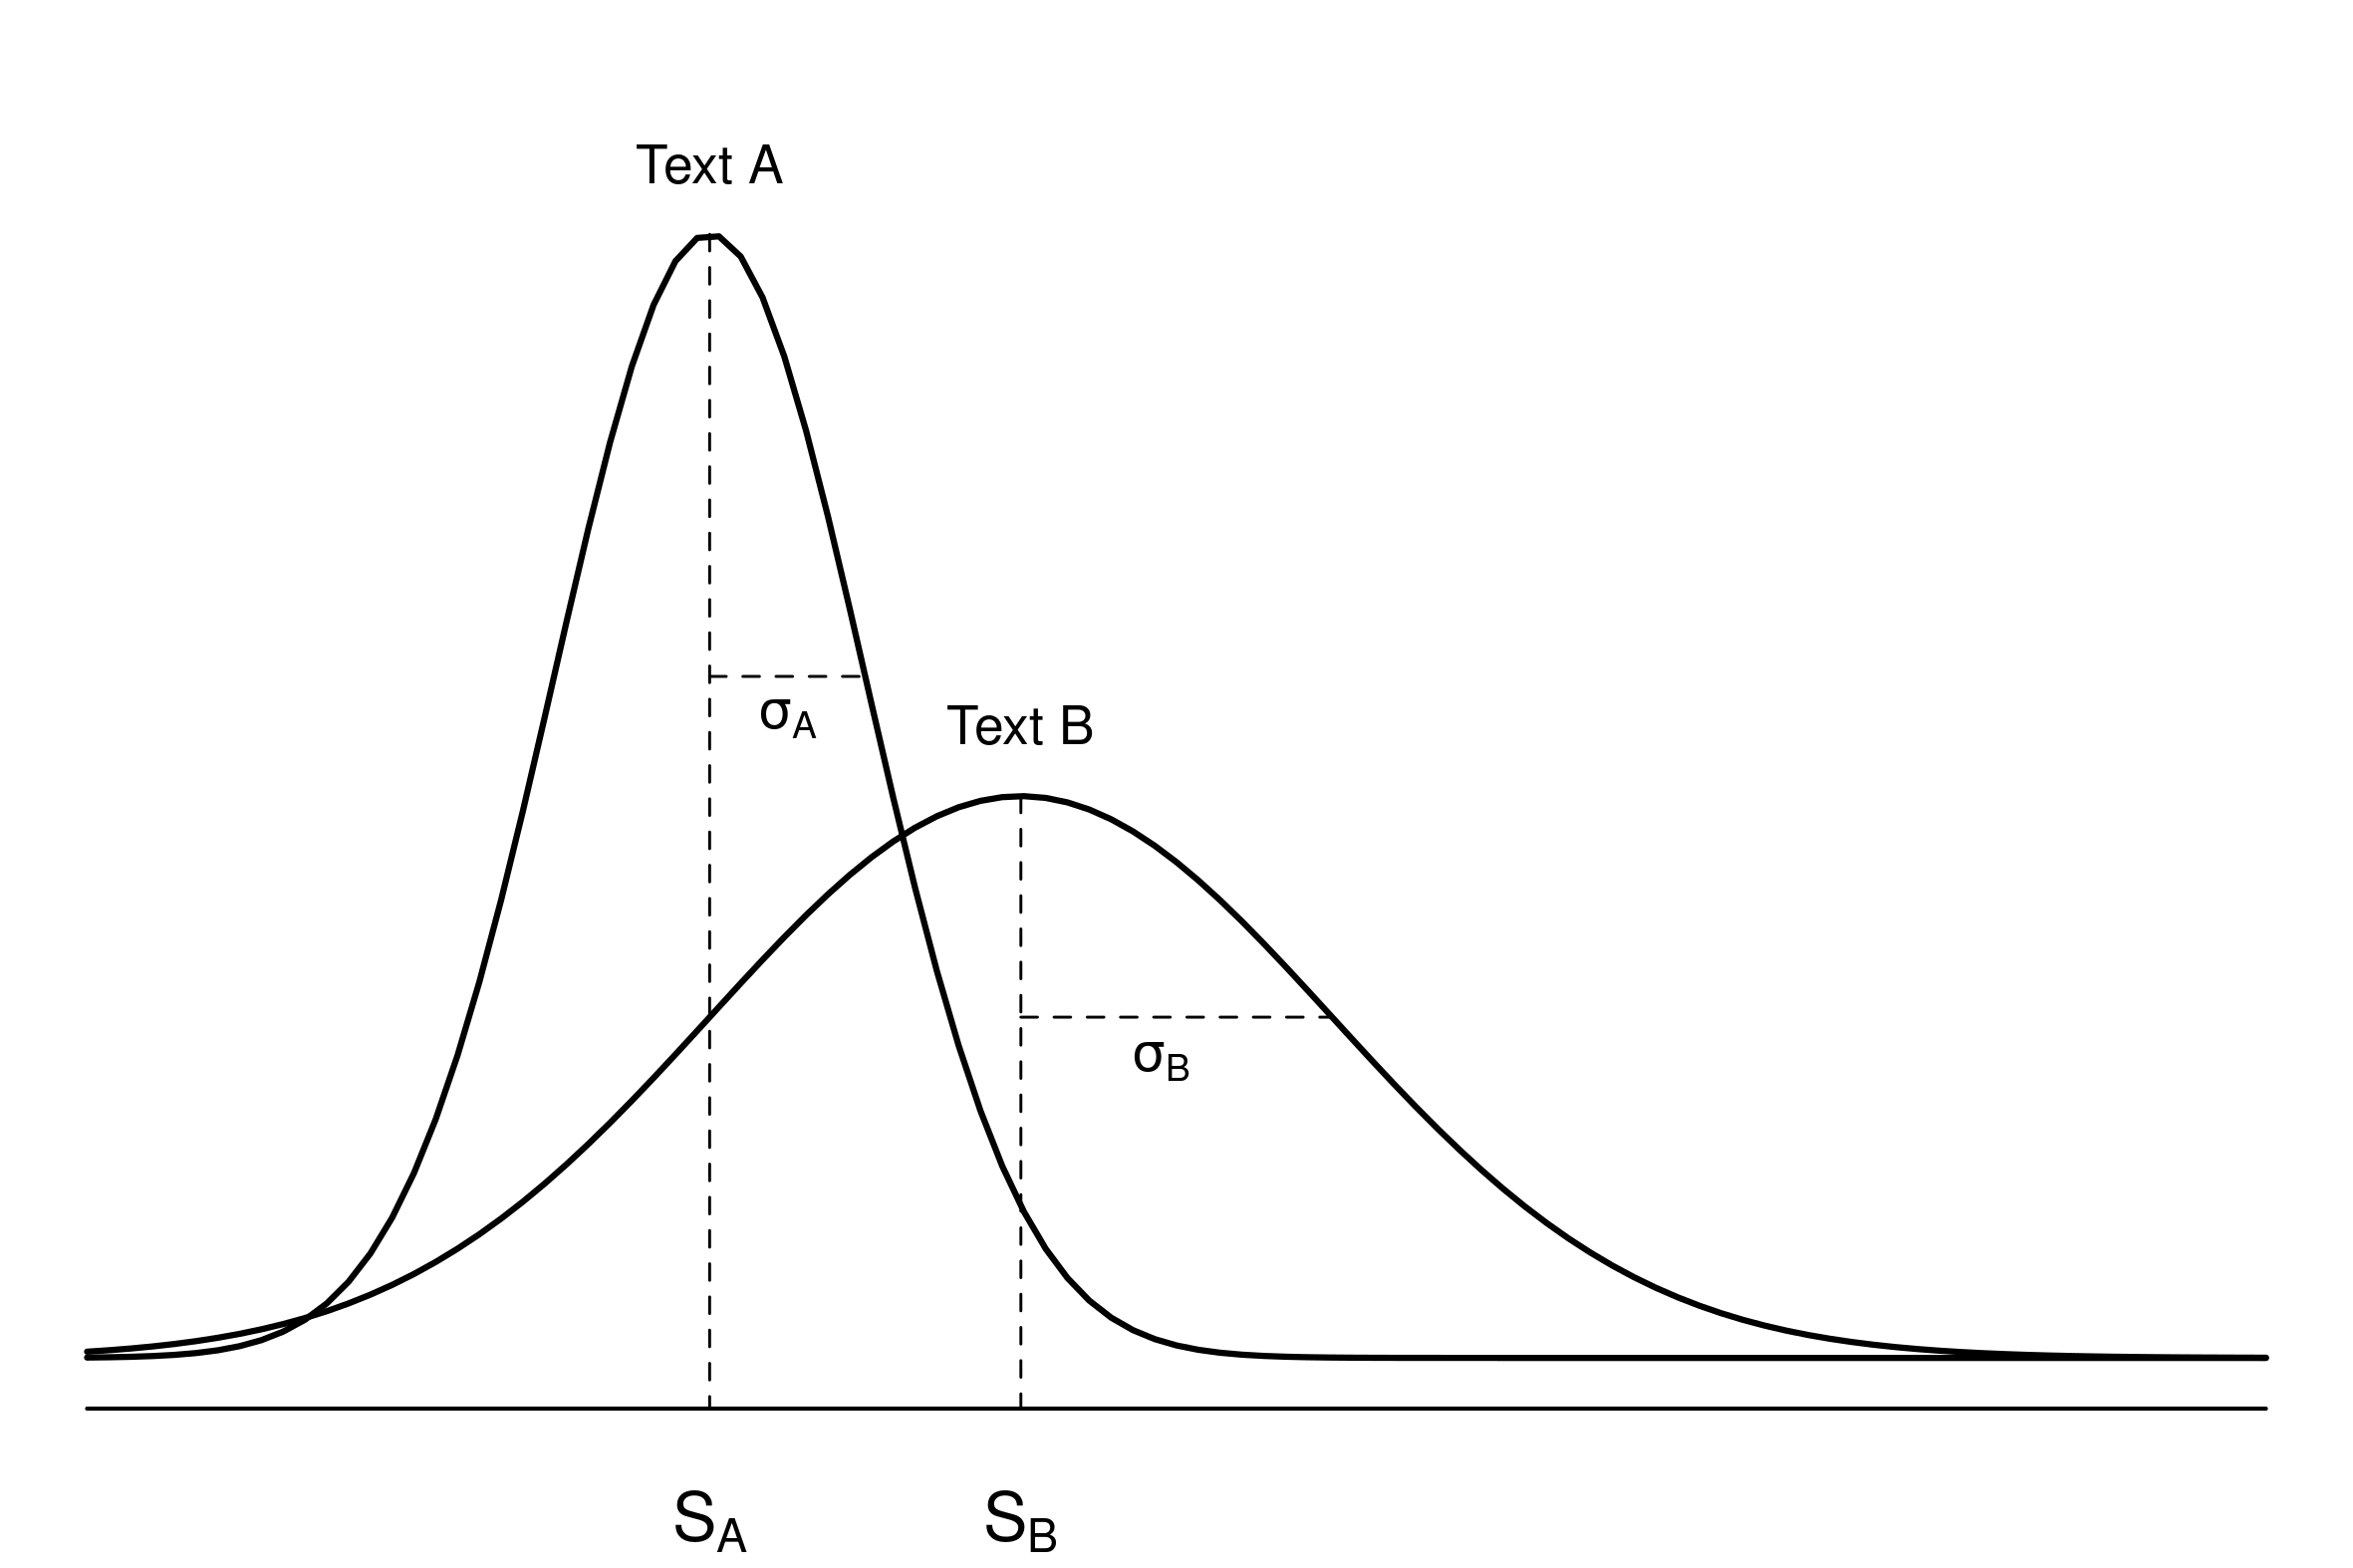
\includegraphics[width=0.95\linewidth,height=\textheight,keepaspectratio]{./images/figures/discriminal_process.png}

}

\subcaption{\label{fig-discriminal_process}Discriminal processes}

\end{minipage}%
%
\begin{minipage}{0.50\linewidth}

\centering{

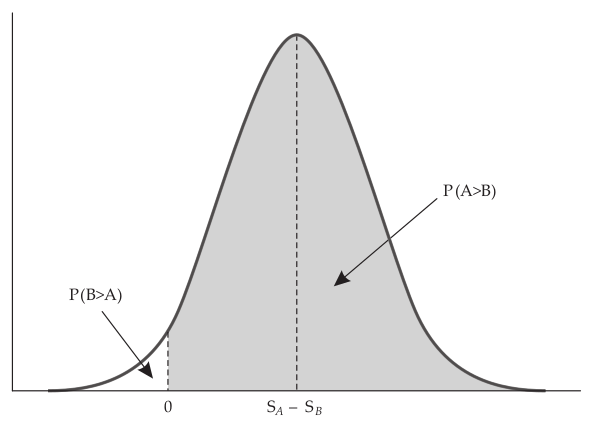
\includegraphics[width=1\linewidth,height=\textheight,keepaspectratio]{./images/figures/comparative_judgment.png}

}

\subcaption{\label{fig-discriminal_difference}Discriminal difference}

\end{minipage}%

\caption{\label{fig-thurstone_theory}Example distribution of discriminal
processes and their discriminal difference for two written texts
(stimuli or objects). Extracted from \citet[pp.~249-251]{Bramley_2008}.}

\end{figure}%

Importantly, the general form of Thurstone's theory primarily addressed
pairwise comparisons of stimuli made by a single judge
\citep[pp.~267]{Thurstone_1927b}. Thus, for practical application,
Thurstone introduced five distinct cases derived from this general form,
each defined by progressively simplifying assumptions.
Table~\ref{tbl-thurstone_cases} summarizes these cases, highlighting key
assumptions such as the distribution of discriminal processes, the
similarity of discriminal dispersions across stimuli, the correlation
between stimuli, and the number of judges performing the comparisons.
For a comprehensive discussion of this progression, refer to
\citet{Thurstone_1927b} and \citet[pp.~248-253]{Bramley_2008}.

\begin{table}

\caption{\label{tbl-thurstone_cases}Thurstones cases and asumptions}

\centering{

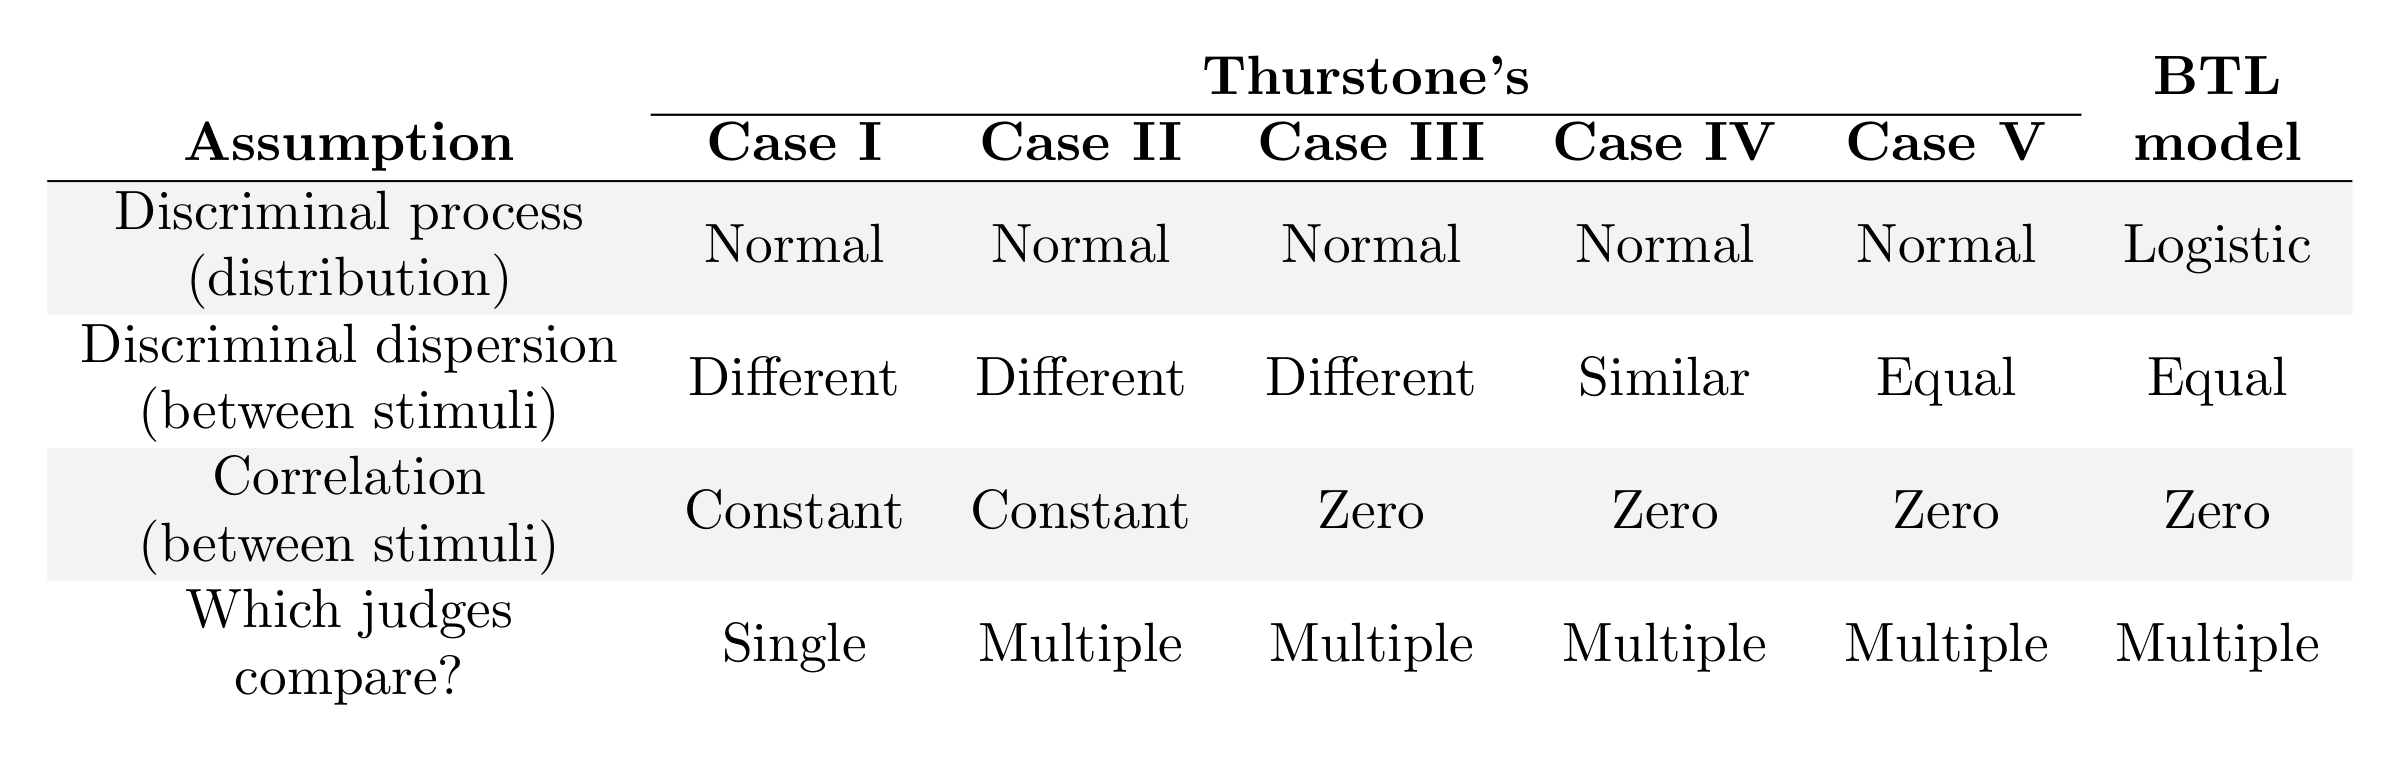
\includegraphics[width=0.9\linewidth,height=\textheight,keepaspectratio]{./images/tables/thurstone_cases.png}

}

\end{table}%

\section{Three critical issues in CJ
literature}\label{sec-theory-issues}

\subsection{The Case V and the statistical analysis of CJ
data}\label{sec-theory-issue1}

Despite its reliance on the largest number of simplifying assumptions
\citetext{\citealp[pp.~253]{Bramley_2008}; \citealp[pp.~677]{Kelly_et_al_2022}},
Case V remains the most widely used case in the CJ literature. This
popularity is largely due to its simplified statistical representation
in the Bradley-Terry-Luce (BTL) model
\citep{Bradley_et_al_1952, Luce_1959}. The BTL model mirrors the
assumptions of Case V, with one key difference: while Case V assumes a
Normal distribution for the discriminal processes of stimuli, the BTL
model uses the more mathematically tractable Logistic distribution
\citep[pp.~254]{Andrich_1978, Bramley_2008} (see
Table~\ref{tbl-thurstone_cases}). This substitution has little impact on
the model's estimation or interpretation, as the Normal and Logistic
distributions share similar statistical properties, differing only by a
scaling factor of approximately \(1.7\)
\citep[pp.~16]{vanderLinden_et_al_2017_I} (see
Figure~\ref{fig-logistic_vs_normal}).

\begin{figure}

\begin{minipage}{0.50\linewidth}

\centering{

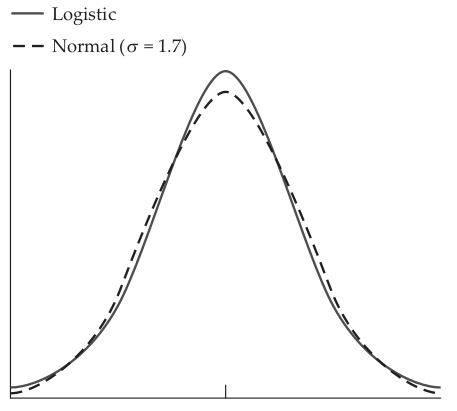
\includegraphics[width=0.85\linewidth,height=\textheight,keepaspectratio]{./images/figures/density.png}

}

\subcaption{\label{fig-density}Probability density}

\end{minipage}%
%
\begin{minipage}{0.50\linewidth}

\centering{

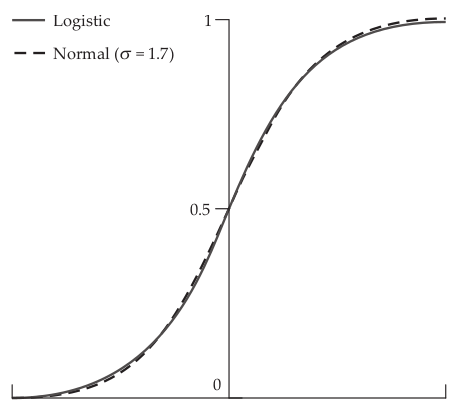
\includegraphics[width=0.85\linewidth,height=\textheight,keepaspectratio]{./images/figures/cumulative.png}

}

\subcaption{\label{fig-cumulative}Cummulative probability}

\end{minipage}%

\caption{\label{fig-logistic_vs_normal}Probability density and
cumulative probability of the logistic and Normal distributions.
Extracted from \citet[pp.~254-255]{Bramley_2008}.}

\end{figure}%

However, Case V was originally developed to provide a ``rather coarse
scaling'' of traits \citep[pp.~269]{Thurstone_1927b}, prioritizing
statistical simplicity over precision in trait measurement
\citep[pp.~677]{Kelly_et_al_2022}. As a result, its assumptions may not
be suitable for applications beyond the psycho-physical contexts for
which it was created. Thurstone himself cautioned that its use ``should
not be made without (an) experimental test''
\citep[pp.~270]{Thurstone_1927b}, acknowledging that some assumptions
could prove problematic in the presence of complex traits or
heterogeneous stimuli, such as handwriting or English compositions
\citep[pp.~374]{Thurstone_1927a}. Consequently, given that modern CJ
applications frequently involve these types of traits and stimuli, two
main assumptions of Case V may not consistently hold in theory or
practice: the zero correlation and equal dispersion between stimuli.

The assumption of \emph{zero correlation between stimuli} can be better
understood through an example. For instance, when using pairwise
comparisons to evaluate text quality, the assumption implies that a
judge's perception of a trait in one text does not influence his
perception of the same trait in another text. Thurstone attributed this
independence to the cancellation of potential judges' biases, driven by
two opposing and equally weighted effects occurring during the pairwise
comparisons \citep[pp.~268]{Thurstone_1927b}. This cancellation was
mathematically demonstrated by \citet{Andrich_1978}, using the BTL model
under the assumption of additive biases in the discriminal processes.
However, it is easy to imagine at least two scenarios where the zero
correlation assumption almost certainly does not hold: when the pairwise
comparison involves multidimensional, complex traits with heterogeneous
stimuli, and when an additional hierarchical structure is relevant to
the stimuli.

In the first scenario, the intricate aspects of multidimensional,
complex traits and heterogeneous stimuli may introduce dependencies
between stimuli. Research on text quality suggests that when judges
evaluate these traits, they often rely on various intricate aspects of
the stimuli to form their judgments
\citep{vanDaal_et_al_2016, Lesterhuis_2018, Chambers_et_al_2022}. In
this context, it is not inconceivable that these aspects, being neither
equally weighted nor opposing, may unevenly influence judges'
perceptions, resulting in biases that resist cancellation. For example,
this might occur when a judge assessing the argumentative quality of a
text places disproportionate emphasis on grammatical accuracy,
ultimately favoring texts with fewer errors but weaker arguments. While
direct evidence for this specific scenario is lacking, studies such as
\citet{Pollitt_et_al_2003} demonstrate the presence of judges' biases,
supporting the idea that the different factors influencing pairwise
comparisons may not always cancel out.

In the second scenario, the shared context or inherent connections
created by the additional hierarchical structure may introduce
dependencies between stimuli, a statistical phenomenon commonly known as
clustering \citep{Everitt_et_al_2010}. Nevertheless, despite recognizing
such hierarchical structures in CJ data, the statistical handling of
this extra source of dependency in the CJ literature has been
inadequate. For instance, in cases where the CJ data included multiple
samples of stimuli from the same individuals, researchers have often
relied on (averaged) estimated BTL scores to conduct subsequent analyses
and tests at the individual hierarchical level
\citep{Bramley_et_al_2019, Boonen_et_al_2020, Bouwer_et_al_2023, vanDaal_et_al_2017, Jones_et_al_2019, Gijsen_et_al_2021}.
This approach, however, has the significant limitation of ignoring the
uncertainty associated with the scores (refer to section
Section~\ref{sec-theory-issue2} for a detailed discussion of this
issue).

In contrast, the assumption of \emph{equal dispersion between stimuli}
suggests that the variability in the perceived trait level of the
stimuli is the same across stimuli. While Thurstone acknowledged that
this assumption may be violated when ``dealing with less conspicuous
attributes or with less homogeneous stimuli''
\citep[pp.~374]{Thurstone_1927a}, no study explicitly proposes that this
assumption could also be violated due to the presence of an additional
hierarchical (grouping) structure relevant to the texts. One such
scenario might arise, for example, when comparing texts produced by
university and secondary school students. In this case, university
students may consistently (or more precisely) produce higher-quality
texts, while secondary school students, who exhibit a broader range of
writing abilities, would show greater variability in the quality of
their texts. Although this example is somewhat contrived, it effectively
illustrates how assuming equal dispersions across texts can overlook
meaningful differences in the reliability of text quality across groups
or individuals.

{``however'' paragraph}

{``to mitigate'' paragraph}

\subsection{The disconnect between trait measurement and hypothesis
testing}\label{sec-theory-issue2}

Building on the previous section, it is evident that the BTL model
commonly functions as the trait's measurement model in CJ experiments
\citep{Andrich_1978, Bramley_2008}. A measurement model specifies how
manifest variables contribute to the estimation of latent variables
\citep{Everitt_et_al_2010}. For example, when evaluating text quality,
researchers use the BTL model to process the dichotomous outcomes
resulting from the pairwise comparisons (the manifest variables) to
estimate scores that reflect the underlying quality level of texts (the
latent variable)
\citep{Laming_2004, Pollitt_2012b, Whitehouse_2012, vanDaal_et_al_2016, Lesterhuis_2018_thesis, Coertjens_et_al_2017, Goossens_et_al_2018, Bouwer_et_al_2023}.

Researchers then typically use the estimated BTL scores, or their
transformations, to conduct additional analyses and tests, or to make
decisions regarding the exclusion of certain data in these analyses and
tests. The literature shows that these scores have been employed to
calculate correlations with other assessment methods
\citep{Goossens_et_al_2018, Bouwer_et_al_2023} or to test hypotheses
related to the underlying traits of interest
\citep{Bramley_et_al_2019, Boonen_et_al_2020, Bouwer_et_al_2023, vanDaal_et_al_2017, Jones_et_al_2019, Gijsen_et_al_2021}.
Additionally, the BTL scores have been used to detect biases in judges'
ratings \citep{Pollitt_et_al_2003, Pollitt_2012b}, as well as to
identify ``misfit'' judges and stimuli
\citep{Pollitt_2012b, vanDaal_et_al_2017, Goossens_et_al_2018}, with
considerations for their possible exclusion.

However, the statistical literature advises caution when using estimated
scores for additional analyses and tests, as well as when eliminating
data through ad hoc univariate procedures. A key consideration is that
BTL scores are parameter estimates that inherently carry uncertainty.
Ignoring this uncertainty can bias the analysis and reduce the precision
of hypothesis tests. Notably, the direction and magnitude of such biases
are often unpredictable. Results may be attenuated, exaggerated, or
remain unaffected depending on the degree of uncertainty in the scores
and the actual effects being tested
\citetext{\citealp[pp.~25]{Kline_et_al_2023}; \citealp[pp.~137]{Hoyle_et_al_2023}}.
Moreover, excluding data using ad hoc univariate procedures can compound
these issues by discarding potentially valuable information, further
exacerbating the bias \citep{Zimmerman_1994, McElreath_2020}. Finally,
the reduced precision in hypothesis tests diminishes their statistical
power, increasing the likelihood of committing type-I or type-II errors
\citep{McElreath_2020}.

To mitigate these risks, principles from Structural Equation Modeling
(SEM) \citep[pp.~138]{Hoyle_et_al_2023} and Item Response Theory (IRT)
\citetext{\citealp[chap.~6]{Fox_2010}; \citealp[chap.~24]{vanderLinden_et_al_2017_I}}
recommend conducting these analyses and tests within a structural model.
A structural model specifies how different manifest or latent variables
influence the latent variable of interest \citep{Everitt_et_al_2010}.
This approach allows analyses that can account for both the BTL scores
and their uncertainties simultaneously, rather than treating them as
separate elements. Therefore, an integrated approach that combines CJ's
measurement and structural models can offer significant advantages.

\subsection{The diverse assessment design features and their role on
reliability and validity}\label{sec-theory-issue3}

\section{An updated theoretical and statistical model for
CJ}\label{sec-theory}

\subsection{The theoretical model}\label{sec-theory-theoretical}

\subsection{From theory to statistics}\label{sec-theory-statistics}

\section{Discussion}\label{sec-discuss}

\subsection{Findings}\label{sec-discuss-finding}

\subsection{Limitations and further
research}\label{sec-discuss-limitations}

\section{Conclusion}\label{sec-conclusion}

\newpage{}

\section*{Declarations}\label{declarations}
\addcontentsline{toc}{section}{Declarations}

\textbf{Funding:} The project was founded through the Research Fund of
the University of Antwerp (BOF).

\textbf{Financial interests:} The authors have no relevant financial
interest to disclose.

\textbf{Non-financial interests:} The authors have no relevant
non-financial interest to disclose.

\textbf{Ethics approval:} The University of Antwerp Research Ethics
Committee has confirmed that no ethical approval is required.

\textbf{Consent to participate:} Not applicable

\textbf{Consent for publication:} All authors have read and agreed to
the published version of the manuscript.

\textbf{Availability of data and materials:} No data was utilized in
this study.

\textbf{Code availability:} All the code utilized in this research is
available in the digital document located at:
\url{https://jriveraespejo.github.io/paper2_manuscript/}.

\textbf{AI-assisted technologies in the writing process:} The authors
used ChatGPT, an AI language model, during the preparation of this work.
They occasionally employed the tool to refine phrasing and optimize
wording, ensuring appropriate language use and enhancing the
manuscript's clarity and coherence. The authors take full responsibility
for the final content of the publication.

\textbf{CRediT authorship contribution statement:}
\emph{Conceptualization:} S.G., S.DM., T.vD., and J.M.R.E;
\emph{Methodology:} S.DM., T.vD., and J.M.R.E; \emph{Software:}
J.M.R.E.; \emph{Validation:} J.M.R.E.; \emph{Formal Analysis:} J.M.R.E.;
\emph{Investigation:} J.M.R.E; \emph{Resources:} S.G., S.DM., and T.vD.;
\emph{Data curation:} J.M.R.E.; \emph{Writing - original draft:}
J.M.R.E.; \emph{Writing - review and editing:} S.G., S.DM., and T.vD.;
\emph{Visualization:} J.M.R.E.; \emph{Supervision:} S.G. and S.DM.;
\emph{Project administration:} S.G. and S.DM.; \emph{Funding
acquisition:} S.G. and S.DM.

\newpage{}

\section{Appendix}\label{sec-appendix}

\newpage{}

\section*{References}\label{references}
\addcontentsline{toc}{section}{References}

\renewcommand{\bibsection}{}
\bibliography{references.bib}





\end{document}
